\section*{Question 4: Perceptrons}



\subsection*{a)}
\begin{figure}[H]
\caption{Single Perceptron}
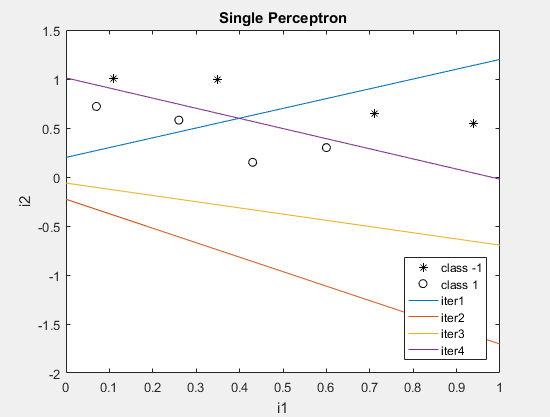
\includegraphics[width=8cm]{singleperc.png}
\centering
\end{figure}

\lstset{frame=tb,
  language=Python,
  aboveskip=3mm,
  belowskip=3mm,
  showstringspaces=false,
  columns=flexible,
  basicstyle={\small\ttfamily},
  numbers=none,
  numberstyle=\tiny\color{gray},
  keywordstyle=\color{blue},
  commentstyle=\color{dkgreen},
  stringstyle=\color{mauve},
  breaklines=true,
  breakatwhitespace=true,
  tabsize=3
}

\begin{lstlisting}[float=h,frame=tb,caption=Perceptron Code,label=zebra]
from random import choice
from numpy import array, dot, random

unit_step = lambda x: -1 if x < 0 else 1

training_data = [
    (array([1,0.1,0.72]), -1),
    (array([1,0.15,1.01]), 1),
    (array([1,0.25,0.55]), -1),
    (array([1,0.32,0.95]), 1),
    (array([1,0.45,0.12]), -1),
    (array([1,0.6,0.3]), -1),
    (array([1,0.7,0.6]), 1),
    (array([1,0.9,0.4]), 1),
]

w = [0.2, 1, -1]
errors = []
eta = 1
epoch = 5

print("Initial Weights: " + str(w))
for z in range(epoch):
    print("Epoch: " + str(z + 1))
    for i in xrange(len(training_data)):
        x, expected = training_data[i]
        result = dot(w, x)
        error = expected - unit_step(result)
        errors.append(error)
        w += eta * error * x
    print("Updated weights: " + str(w))
    tmp_err = 0
    for l in range(len(training_data)):
        x, expected = training_data[l]
        result = dot(w, x)
        if expected != unit_step(result):
            tmp_err = tmp_err + 1
    print("Missclassified: " + str(tmp_err))
\end{lstlisting}

\begin{lstlisting}[float=h,frame=tb,caption=Code output,label=zebra]
Epoch: 1
Updated weights: [ 0.2   1.3   0.88]
Missclassified: 4
Epoch: 2
Updated weights: [ 0.2   2.04  3.22]
Missclassified: 4
Epoch: 3
Updated weights: [-1.8   1.84  1.78]
Missclassified: 0
Epoch: 4
Updated weights: [-1.8   1.84  1.78]
Missclassified: 0
\end{lstlisting}

By iteration 4 all the points were being perfectly classified.

\clearpage
\subsection*{b)}
The perceptron perfectly classified the set of points.

\subsection*{c)}

\begin{figure}[H]
\caption{Single layer perceptrons}
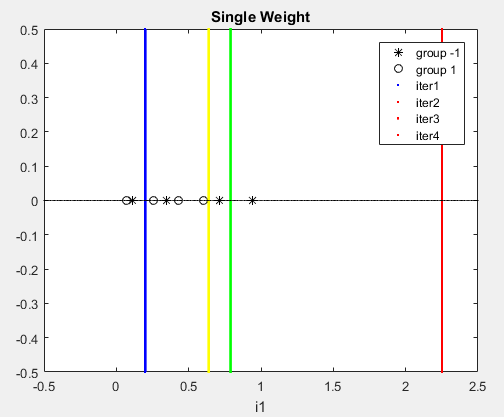
\includegraphics[width=8cm]{svmlin.png}
\centering
\end{figure}

The best we can linearly separate the data points without $i_2$ is 2 classification errors. 
We get $b = -1.8$ and $w_1 = 2.82$ making the point it separates at $i_0$ = 0.63 